\documentclass[../main.tex]{subfiles}


\begin{document}

\chapter{Protocol design}
\label{chap:design}

This chapter describes and justifies the protocol designed in the context of this thesis.
The main purpose of the protocol is the secure encryption of logs in the toolchain.
In the previous chapter \ref{chap:overview}, possible encryption strategies were introduced and evaluated based on the identified system requirements (see chapter \ref{chap:requirements}).
Hybrid encryption was identified as the most promising encryption technique.
The evaluation of the protocol in terms of functionality, security, and performance can be found in chapter~\ref{chap:evaluation}.

A high-level overview of the designed protocol can be found in section~\ref{sec:overview}.
Section~\ref{sec:protocol-considerations} reflects different design considerations for the protocol.
The imposed algorithms to create, encrypt and decrypt logs are explained in the subsequent sections. 

\section{Protocol overview}
\label{sec:overview}

The implemented protocol extends the current toolchain because it supports encrypted logs.
Additionally, access to encrypted logs can be shared and revoked by the data owner.

The protocol relies on an established PKI.
Each user requires two key pairs.
The first key pair is dedicated to encrypting data.
Its public key is called encryption key while its private key is called decryption key.
The second key pair is intended to sign data.
Its public key is called verification key while its private key is called signing key.
Public keys are represented by a PEM-encoded certificate which is signed by a trusted CA.
Private keys are represented by a PEM-encoded private key.
This separation of keys is considered to be the best practice in modern key management.~\todo{quelle}
Each user needs to have exclusive access to its private keys.
The public keys of all users are expected to be publicly available in the system.
The protocol further assumes that a user that participates in the system has access to its key material (e.g. via hardware token).

The protocol relies on three fundamental cryptographic operations:
Signing, encrypting and decrypting logs.
They are used to construct the full functionality of the demanded protocol.
They allow the E2EE of logs and they can be used to share and revoke access to logs.
The following description delivers a high-level overview of how the protocol functions.
This is additionally visualized in figure~\ref{fig:protocol-overview}.

\begin{enumerate}
    \item
    Whenever a monitor component observes a data access it is required to create an access log.
    A log must always be a signed data structure.
    Thus, the protocol requires the monitor to perform two tasks.
    First, the raw log data needs to be cryptographically signed by the monitor.
    Second, the log needs to be encrypted for the data owner (only the data owner is allowed to access the log upon creation).
    The encrypted log is finally sent to the Overseer.
    This allows the data owner to request and decrypt the log.
    The decryption process also involves validity checks of the received data.
    This ensures that the protocol was applied correctly.
    \item 
    The data owner can share or revoke access to a log for users.
    First, the data owner needs to download and decrypt the log from the server.
    To share or revoke access the data owner then needs to apply the encryption algorithm with a set of desired users.
    Please note that the decrypted log stores information about the users who are currently allowed to access the log.
    Access can be shared by adding additional users during encryption.
    Access can be revoked by omitting users during encryption.
    It is crucial to the protocol that the data owner always specifies itself within the set of authorized users.
    Otherwise, the data owner can not decrypt the log anymore.
    Finally, the user uploads the log to the server.
    \item
    Users who are specified during a sharing process can download and decrypt the corresponding log.
    They can request the server for those logs and apply their private decryption key to restore the plain log.
    Again, validity checks of the received data ensure that the defined security requirements are respected.
    
\end{enumerate}

Please note that the encryption algorithm can be applied by the monitor and the owner of the log.
Although only data owners are allowed to share and revoke access to logs, the log must be initially made available for the data owner.
This can be done by encrypting the log only for the data owner:
Whenever a monitor created and signed a new log it applies the encryption algorithm.
The only recipient for this new log must be the data owner.
To ensure that the monitor does not specify other unintended users, validation checks during decryption are mandatory.

\begin{figure}[h!]
    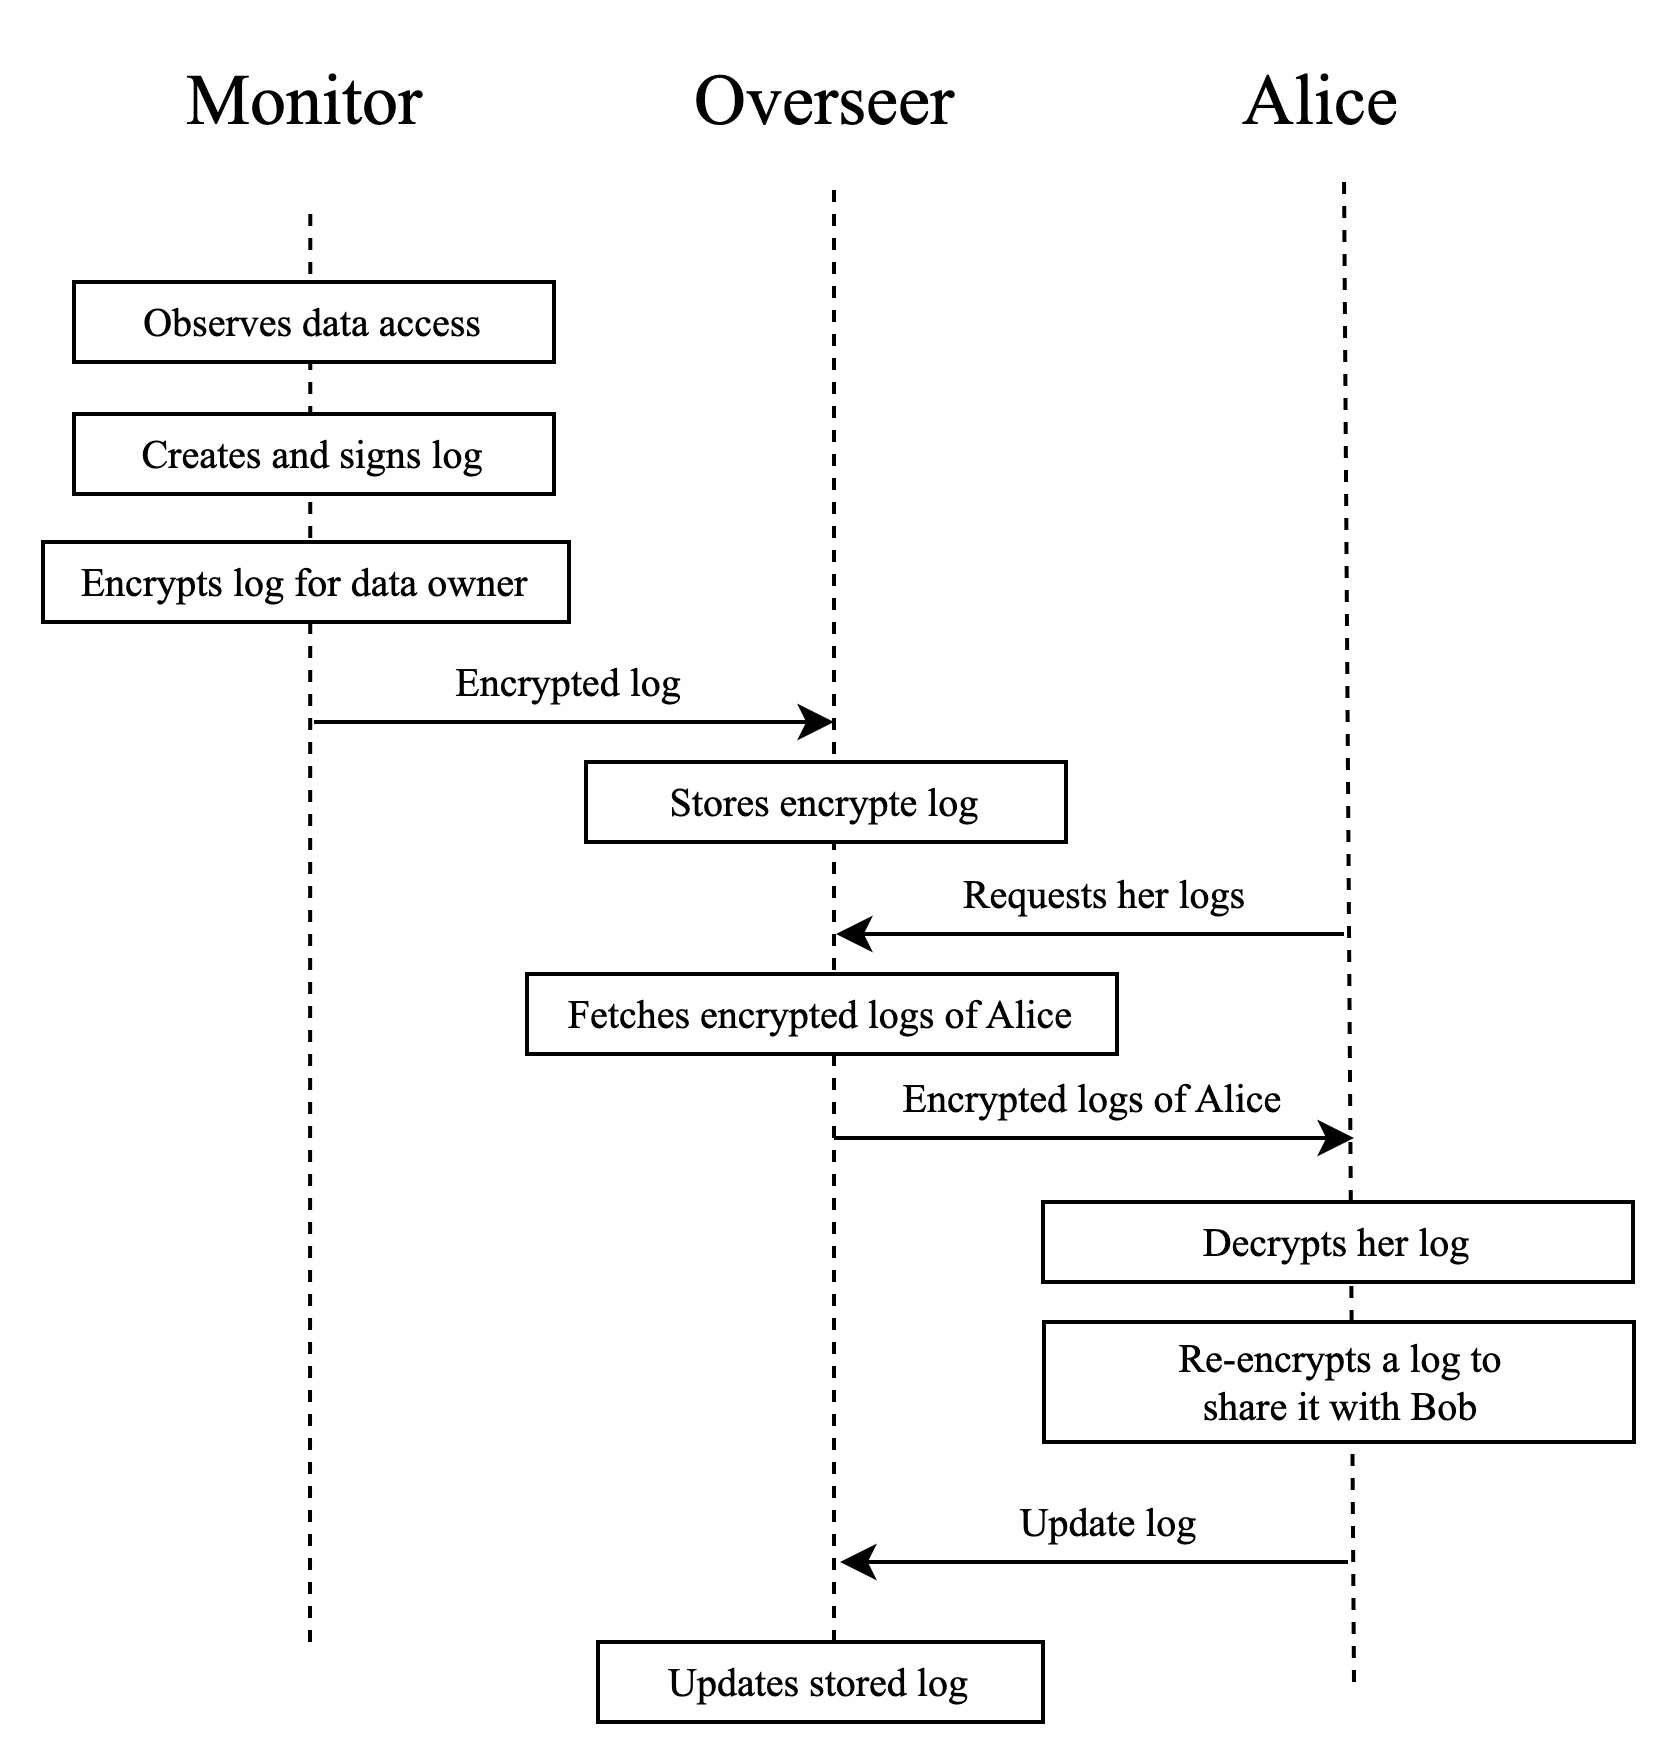
\includegraphics[width=10cm]{../img/05/overview.jpg}
    \centering
    \caption{
        The performed tasks and data flows when creating, encrypting, decrypting and sharing logs in the toolchain.
        The monitor creates a log and encrypts it for Alice.
        Alice downloads and decrypts the log.
        Alice decides to share the log with Bob.
        Therefore, Alice re-encrypts the log and updates it in the Overseer.
        Revoking Bob's access requires Alice to re-encrypt the log while not including Bob into the set of recipients.
    }
    \label{fig:protocol-overview}
\end{figure}

\section{General considerations}
\label{sec:protocol-considerations}
In this section, general design considerations for the protocol are discussed.
Section~\ref{sec:sign-and-encrypt} evaluates the secure combination of encryption and authentication mechanisms.
To design a practical and efficient protocol, intermediate servers are dependent on metadata.
This is elaborated in section~\ref{sec:metadata}.
Finally, section~\ref{sec:jose-protocol} illustrates how the \emph{JOSE} standard can be used to practically implement the protocol.

\subsection{Secure application of encryption and authentication}
\label{sec:sign-and-encrypt}
In general, the protocol sends encrypted data (containing a log) to a set of recipients.
The recipients must verify the authenticity of the encrypted data because only the owner or the monitor of a log can encrypt.
Thus, the creator of an encrypted log is required to cryptographically sign the sent data.
This arises the question, if encrypted data should be signed (\emph{encrypt-then-sign}) or if signed data should be encrypted (\emph{sign-then-encrypt}).
In general, the \emph{encrypt-then-sign} approach is considered less secure because a malicious entity could simply stripe the signature and sign the ciphertext using its own secret key~\cite{Davis2001}.
This might lead to unintended flaws in the resulting protocol~\cite[section~11.2]{Jones2015a}.

The naive \emph{sign-then-encrypt} approach, however, suffers from surreptitious forwarding in certain scenarios (details in section~\ref{sec:surreptitious-forwarding}).
The use case of this protocol is affected by the flaw.
Consider a log which is signed by the data owner indicating that he intentionally shared it.
This signed log is then encrypted for a set of users.
Assume that a malicious user can decrypt the cipher because the data owner encrypted the log for him.
Nothing prevents him from re-encrypting the singed log for any other users.
The problem arises because those other users can not verify if the data owner has intended to share the log with them.
They only know that the log was singed by the data owner.

This flaw can be mitigated by explicitly signing the intended recipients.
This allows a recipient to ensure that the data was intentionally encrypted for him or her by the claimed creator.~\cite{Davis2001}

For the protocol designed in the context of this thesis, those considerations have the following implications:
\begin{enumerate}
    \item 
    The creator of a encrypted log signs the log along with the set of recipients.
    Please note that the log itself is also a signed data structure.
    The log must always be signed by the monitor specified within the log to avoid the forgery of logs (security requirement~S3).
    The signature of the creator ensures that unauthorized sharing operations can be detected (security requirement~S2).
    This construction nests singed data structures into each other.
    Details can be found in section~\ref{sec:encrypting}.
    \item 
    The signed data is then encrypted for the specified recipients.
    This produces the ciphertext which can only be decrypted by those recipients (security requirement~S1).
\end{enumerate}


\subsection{Metadata}
\label{sec:metadata}
The logs which are exchanged between users are always encrypted.
This affects the performance of the toolchain.
From the perspective of intermediate servers, a encrypted log does not provide any meaningful information.
Specifically, they do not know which users have access to a log.
The server can not associate users with a log.
This introduces the following practical problems:
\begin{enumerate}
    \item 
    Consider that Alice requests the logs concerning her.
    If the server can not associate logs with users, it must reply with all logs stored in the system.
    As a consequence, Alice receives many logs that she can not decrypt.
    Since the raw cipher does not tell her which logs are intended for her, Alice must try to decrypt all logs to find the logs encrypted under her public key.
    This is very inefficient and requires a lot of computational power.
    To avoid this, the set of recipients can be attached as metadata to the encrypted log.
    \item 
    Consider Alice to be a data owner.
    Alice wants to share her log with Bob.
    Before the sharing process starts, the encrypted log is stored in the server.
    Alice re-encrypts the log under the public key of Bob.
    She authenticates against the server and tries to update the stored log in the server.
    The server, however, does not know if Alice is the legitimate owner of the stored log (because it can not associate users with a log).
    Thus, the server can not allow Alice to update the stored log.
    To avoid this, the server must know the identities of the data owners for all logs.
    This can be realized by attaching the identity of the owner as metadata to the encrypted log.
\end{enumerate}
To avoid these problems, the set of receivers and the identity of the data owner need to be accessible without decryption.
This data can be interpreted as routing information and must be attached as metadata to the encrypted logs.
This allows the server to filter logs which concern a particular user.
Moreover, the server can allow data owners to modify encrypted logs.
This practically allows them to share and revoke access to logs.
This construction, however, implies that the data sent over the insecure network contains the set of recipients twice (once in the metadata and once within the encrypted data).

\subsection{Realization via JOSE}
\label{sec:jose-protocol}

A log within the current inverse transparency toolchain is represented by a json object.
This motivates the usage of the \emph{JSON Object Signing and Encryption} standard (\emph{JOSE})~\cite{Barnes2014}.
Details about it can be found in section~\ref{sec:jose}.
The \emph{JOSE} standard can be used to cryptographically sign (\emph{JWS}) and encrypt (\emph{JWE}) json data.
It defines multiple algorithms which can be used.
Specifically, \emph{JWE} tokens can be computed using hybrid encryption algorithms.
Since \emph{JWS} and \emph{JWE} tokens can also be nested into each other, \emph{JOSE} cab be used to realize the desired protocol by the following means:
\begin{enumerate}
    \item 
    A log is a \emph{JWS} token signed by the monitor.
    \item 
    To encrypt a log, the creator computes a \emph{JWS} token which contains the log as a nested token.
    The token additionally contains the set of intended recipients.
    This outer \emph{JWS} token is called a shared log in the context of this protocol.
    See figure~\ref{fig:nested-jws} for a visualization of the nested tokens.
    \item
    The shared log is finally encrypted to obtain a \emph{JWE} token.
    This token also contains the unencrypted metadata within its protected header.
\end{enumerate}


\begin{figure}[h!]
    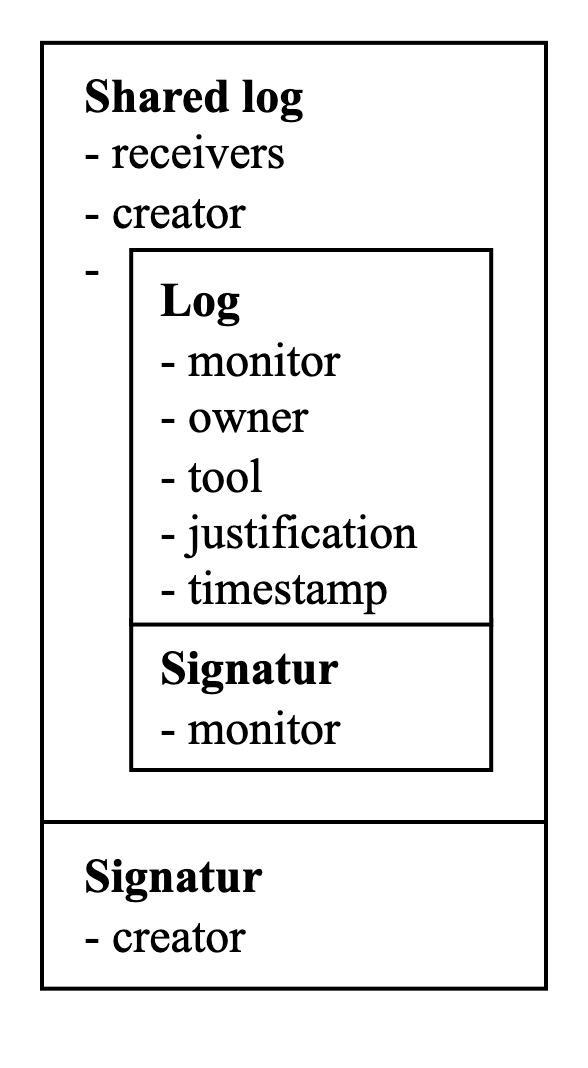
\includegraphics[width=4cm]{../img/05/nested_jws.jpg}
    \centering
    \caption{A log is a \emph{JWS} token signed by the monitor. A shared log is a \emph{JWS} token that contains a nested log. It is signed by the entity encrypting the log.}
    \label{fig:nested-jws}
\end{figure}




\section{Creating logs}
\label{sec:signing}
A log is represented by a \emph{JWS} token.
It contains the identity of the owner, the identity of the monitor and further information which are relevant to identify the data access (see figure~\ref{fig:nested-jws}).
To avoid malicious data owners manipulating or creating new logs, each log needs to be signed by the monitor specified within the log.
To create a \emph{JWS} token, the monitor requires access to its private signing key.
A log is signed with the algorithm \verb|ES256| which relies on \verb|ECDSA| and \verb|SHA-256|.
It is defined by the JSON Web Algorithm specification~\cite{Jones2015}.
The log is later used as input for the encryption algorithm.
This construction is intended to resolve security requirement S3 because allows users decrypting a log to verify if the provided log was indeed created by the claimed monitor.

\section{Encrypting logs}\label{sec:encrypting}

The encryption algorithm requires two input parameters: A log and the set of users who are allowed to access the log.
It can be performed either by a monitor or the data owner.
A monitor initially encrypts the log for the data owner.
The monitor must not include its own identity into the set of authorized users.
More specifically, the set of authorized users must only contain the data owner if a monitor initially encrypts a log.
The data owner of the log might decide to share or revoke access to a log for users later on.
This requires the re-encryption of the log.
The data owner must always include its own identity into the set of authorized users.
The encryption algorithm outputs a \emph{JWE} token which can be decrypted by the specified users.

Internally, the encryption algorithm creates another \emph{JWS} token.
This token is signed with the private signing key of the user encrypting the log (e.g. the creator).
It is called a shared log because it contains a nested log plus the set of recipients plus the identity of the creator (see figure~\ref{fig:nested-jws}).
The latter allows a decrypting user to download the public key of the creator which is used to verify the shared log.
The set of recipients is included to mitigate surreptitious forwarding.
This construction is intended to resolve security requirement S2.
It allows to verify a receiver if the data owner has intended to share the log with him or her.
 
Once the  shared log is created, it is used to compute the final \emph{JWE} token.
This follows the \emph{sign-then-encrypt} approach elaborated in section~\ref{sec:sign-and-encrypt}.
The final token is computed by passing the encoded shared log as plaintext into the \emph{JWE} encryption algorithm.
The identities of recipients and the identity of the owner are passed as metadata into the protected header of the \emph{JWE} token.
The choice of used algorithms to encrypt the data implies hybrid encryption:
The plaintext is encrypted with the authenticated encryption algorithm \verb|A256GCM| (symmetric encryption via 256-bit AES in Galois/Counter Mode).
The applied key-wrapping algorithm is \verb|ECDH-ES+A256KW|.
It is responsible computing encrypted keys.
For each user specified as valid recipient, the symmetric key is encrypted under the public encryption key of the user (asymmetric encryption).
This algorithm establishes a Diffie-Hellman secret between the creator and recipient.
This DH-secret is finally used to encrypt the symmetric key using AES.
Details about this approach can be found in \cite[100]{Barker2017}.
Both algorithms are specified by the JSON Web Algorithm specification~\cite{Jones2015}.
The resulting \emph{JWE} token contains the symmetrically encrypted log, all encrypted keys, and the protected header.
It can only be decrypted by the specified recipients because they are the only users who can restore the symmetric encryption key.
This is intended to resolve security requirement S1 because it effectively end-to-end encrypts a log.
The whole encryption process is depicted in detail in the appendix~\ref{app:encryption}.

\section{Decrypting logs}\label{sec:decrypting}

The decryption algorithm takes a \emph{JWE} token and a private decryption key as input.
To verify the \emph{JWS} tokens encoded within the \emph{JWE} token, this algorithm needs to be able to dynamically resolve the identities of users to their public keys.

First of all, the \emph{JWE} token is parsed into its ciphertext, header and encrypted keys.
The \emph{JWE} decryption algorithm is then applied to the cipher.
This decrypts the ciphertext using the passed private decryption key.
To be more precise, it tries to decrypt any of the encrypted keys provided by the \emph{JWE} token.
If this succeeds, the symmetric encryption key is accessible.
This allows the decryption of the symmetric ciphertext which restores the shared log.
No decryption is necessary to access the metadata because is stored in the protected header of the \emph{JWE}.

If the decryption is successful, the decrypting user has access to the shared log and the metadata.
Multiple validations are necessary to ensure that the protocol is used correctly.
If any of them fails the decryption must be aborted.
\begin{enumerate}
    \item 
    The signature of the obtained shared log (outer \emph{JWS} token) must be validated.
    To do so, the decrypting user needs to download the public key of the creator specified in the shared log.
    If the verification of the signatures succeeds, the decrypting user can be sure that the claimed creator indeed signed the shared log.
    \item
    The signature of the nested log (inner \emph{JWS} token) must be validated.
    Again, the public key of the specified monitor needs to be downloaded.
    The PKI must ensure that this public key belongs to a valid and trusted monitor component.
    If the verification of the signatures succeeds, the decrypting user can be sure that the claimed monitor indeed signed the log.
    \item
    The metadata includes the set of recipients.
    The shared log also includes this information.
    Only if both sets are equal the token was not modified during transit.
    \item
    The user applying the decryption must be part of the set of recipients.
    If this is true, the user can ensure that the creator intended to share the log with him or her.
    \item
    The owner specified in the metadata must be equal to the owner specified in the log.
    Only if both are equal the token was not modified during transit.
    \item
    The log specifies the owner and the monitor of the log.
    The shared log specifies the creator of the encrypted message.
    The creator must be either the owner or the monitor of the log.
    
    If the creator is equal to the monitor of the log, the monitor encrypted the message for the data owner.
    In this case, the decrypting user must be the data owner.
    The set of recipients must only contain the identity of the data owner because the monitor is not allowed to encrypt the log for other users.

    On the other hand, the creator can be equal to the owner of the log.
    This implies that the owner shared the log with other users.
    In this case, the set of recipients can be arbitrary.
\end{enumerate}
If all those validations succeed the log can be trusted.
A visualization of the decryption process can be found in the appendix~\ref{app:encryption}

\end{document}
